%% Manuscript draft: per-powder calibration of the open-source auger doser
%% as multi-objective, multi-task Bayesian optimization, and dosing response
%% as a probe of powder flow.  Target: Additive Manufacturing (Elsevier),
%% full-length article.  Build: `make` (pdflatex + bibtex, MiKTeX or TeX Live).
%%
%% Conventions used in this draft (remove before submission):
%%   \ph{...}      a value or statement that waits on data not yet collected
%%   [Placeholder] figure captions starting with this tag show synthetic data;
%%                 the figure itself carries a diagonal "SYNTHETIC DATA" mark.
%% Everything else reports work that exists in the repository.
\documentclass[preprint,12pt]{elsarticle}

\usepackage[T1]{fontenc}
\usepackage{lmodern}
\usepackage{amsmath,amssymb}
\usepackage{graphicx}
\usepackage{booktabs}
\usepackage{tabularx}
\usepackage{multirow}
\usepackage[per-mode=symbol]{siunitx}
\usepackage[usenames,dvipsnames]{xcolor}
\usepackage{lineno}
\usepackage[hidelinks]{hyperref}
\usepackage{enumitem}
\usepackage{microtype}

\sisetup{range-phrase=--, range-units=single}
\DeclareSIUnit\rpm{rpm}

% Placeholder marker: a value or claim that waits on data.  Grey box, so it is
% easy to find in the PDF and hard to mistake for a result.
\newcommand{\ph}[1]{\colorbox{orange!18}{\textsf{\footnotesize #1}}}
\newcommand{\phfig}{\textcolor{orange!80!black}{\textsf{[Placeholder: synthetic data.]}}~}

\journal{Additive Manufacturing}

\begin{document}

\begin{frontmatter}

\title{Auger-based powder dosing as a probe of powder flow:\\
multi-objective, multi-task Bayesian calibration and\\
physics-based property inference}

%% Author list and order follow the companion hardware paper and are not yet
%% agreed for this paper (see OUTLINE.md, "Decisions for the authors").
\author[byu]{Will Mulberry}
\author[byu]{Sam Charles}
\author[byu]{Luke Winters}
\author[byu]{Carl Robison}
\author[byu]{Gage Erickson}
\author[byu,ac]{Sterling G. Baird\corref{cor1}}
\ead{sterling.baird@byu.edu}
\cortext[cor1]{Corresponding author.}

\affiliation[byu]{organization={Department of Mechanical Engineering, Brigham Young University},
  city={Provo}, state={UT}, country={USA}}
\affiliation[ac]{organization={Acceleration Consortium, University of Toronto},
  addressline={80 St George St}, city={Toronto}, state={ON}, postcode={M5S 3H6}, country={Canada}}

\begin{abstract}
How much powder an auger delivers depends on how it is driven and on the powder itself, so every calibration of an auger doser is also a small measurement of how that powder flows.
We treat the calibration of an open-source, 3D-printed auger doser as multi-objective Bayesian optimization and ask what the calibration data reveal about the powder.
With fixed settings, 13 powders, from food-safe stand-ins to AlSi10Mg and silicon, moved between 10 and 231~mg per auger revolution, and three moved none.
On sodium chloride, an optimizer tuned eight controller settings unattended in 51 doses and less than 2.5~h, and its recommended settings dosed 0.5~g in 100~s with a 2.4~mg error, against 3 to 6~min for hand-tuned settings.
We extend the formulation to many powders by treating each powder as a related task, so that a multi-task model shares what it learns, and add objectives for repeatability and accessible dose range.
A discrete element model of the auger, run with real grain sizes and no calibration, reproduces the measured delivery per revolution within \ph{12}\% at three of four tilt angles; we use it, with measured particle-size distributions, to infer an effective cohesion and friction for each powder from its dosing response.
\ph{Multi-task calibration cut the doses needed per new powder by X\%, and the inferred parameters tracked Hall-flow and shear-cell measurements (R$^2$ = Y).}
Because the doser already sits in an alloy-discovery workflow, these measurements come at no extra cost and may help anticipate how a feedstock will spread and pack.
\end{abstract}

\begin{graphicalabstract}
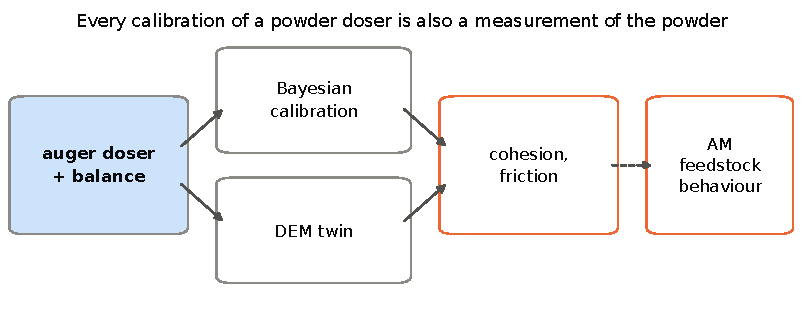
\includegraphics[width=\linewidth]{figures/graphical_abstract}
\end{graphicalabstract}

\begin{highlights}
\item An open-source auger doser is calibrated per powder by Bayesian optimization
\item Eight controller settings were tuned unattended in under 2.5 h on salt
\item Delivery per auger turn spans 24-fold across 13 powders at fixed settings
\item Each powder is a task; multi-task models share data across powders
\item A DEM twin turns dosing data into effective cohesion and friction
\end{highlights}

\begin{keyword}
powder dosing \sep powder flowability \sep Bayesian optimization \sep multi-task learning \sep discrete element method \sep self-driving laboratory
\end{keyword}

\end{frontmatter}

\linenumbers

%% ---------------------------------------------------------------------------
\section{Introduction}
\label{sec:intro}

Alloy discovery by additive manufacturing (AM) starts with weighing powders. Each candidate composition is made by blending elemental or pre-alloyed powders, either in a bed for laser powder bed fusion (L-PBF) or in the feeders of a directed energy deposition (DED) system \cite{Mosallanejad2021Situ,Moorehead2020Throughput,Li2018Combinatorial,Vecchio2021Throughput,Mooraj2024Additive,Nelaturu2024Multi}. In a self-driving laboratory (SDL), where a planning algorithm chooses each next composition and robots make and test it \cite{Abolhasani2023Rise,Tom2024Self,Seifrid2022Autonomous}, that weighing step must be automatic, accurate, and fast for every powder in the palette \cite{Szymanski2023Autonomous,Lunt2024Modular,Jiang2023Autonomous,Maffettone2023What}. The same powders must later spread into thin, uniform layers, and how well they do so depends on the same properties that make them easy or hard to dose: particle size and shape, cohesion, and friction \cite{Vock2019Powders,Meier2019Critical,Brika2020Influence,Haferkamp2021Influence}.

Measuring those properties is slow and often uninformative. Hall and Carney funnels report a single flow time and cannot test cohesive powders, which do not flow through them at all \cite{Spierings2016Powder,Krantz2009Characterization}. Shear cells and powder rheometers give richer data, but each test needs tens of millilitres of powder, a dedicated instrument, and a trained operator \cite{Schulze2021Powders,Freeman2007Measuring}. Rotating drums and spreadability tests come closer to the conditions in an AM machine \cite{Lumay2012Measuring,Yablokova2015Rheological,Snow2019Development,Cordova2020Measuring}, yet different flow tests often rank the same powders differently, and none of them predicts spreading reliably on its own \cite{Spierings2016Powder,Krantz2009Characterization,Snow2019Development}. For an SDL that cycles through dozens of feedstocks, including small batches of reactive or expensive powders, a separate characterization campaign for each powder is rarely affordable.

Powder feeders, by contrast, are characterized all the time, because each new powder must be calibrated before it can be dosed. In pharmaceutical manufacturing, the feed factor of a screw feeder, the mass it delivers per screw revolution, has been predicted from bulk density, compressibility, and shear-cell data \cite{Wang2017Predicting,Tahir2020Development,Bekaert2021Determination}, and loss-in-weight feeders have standard methods for measuring how their output varies \cite{Engisch2012Method,Engisch2015Feedrate,Hanson2018Control}. If material properties predict feeder behaviour, the inverse should also hold: a feeder that is driven through a designed set of conditions, and weighed, measures the powder. Small-scale dosers make this attractive because the measurement uses milligrams to grams of powder and happens anyway, every time a new powder is loaded \cite{Besenhard2015Accuracy,Besenhard2017Micro,Faulhammer2014Dose,Yang2007Metering,Alsenz2011Powderpicking}.

Calibration of this kind is an optimization problem with several competing goals. A dose should be accurate and repeatable, it should be fast, and the settings should work across the range of doses the workflow needs. Overshoot cannot be undone, because powder cannot be taken back out of the cup, so error in one direction costs more than in the other. Bayesian optimization (BO) suits such problems: it fits a probabilistic model to the doses made so far and chooses the next settings where the expected gain is largest \cite{Shahriari2016Taking,Liang2021Benchmarking,Baird2026Honegumi}. Multi-objective BO finds the trade-off, or Pareto front, between goals such as time and error \cite{Daulton2021Parallel}, and sparse priors make it practical with many settings and few experiments \cite{Eriksson2021High}. Each new powder, however, still starts from scratch. Multi-task BO treats related problems, here different powders on the same doser, as tasks of one model, so that data from earlier powders inform the first doses of a new one \cite{Bonilla2008Multi,Swersky2013Multi,Taylor2023Accelerated}. How strongly two powders are related is then a learned quantity, and it is natural to ask whether it reflects their physical properties.

Physics-based models can answer that question directly. The discrete element method (DEM) simulates every grain and its contacts \cite{Cundall1979Discrete,Zhu2008Discrete}, has been used to predict the output of screw conveyors \cite{Owen2009Prediction}, and represents cohesion and rolling friction with contact laws whose parameters are hard to measure \cite{Johnson1971Surface,Thakur2014Micromechanical,Ai2011Assessment}. These parameters are usually calibrated by matching simulations to bulk tests, which is itself an inverse problem \cite{Coetzee2017Review,Richter2020Development,Benvenuti2016Identification,Cheng2019Iterative}, best treated with the tools of Bayesian calibration of computer models \cite{Kennedy2001Bayesian,Higdon2008Computer}. DEM is also the standard tool for studying how powders spread into AM layers \cite{Haeri2017Optimisation,Nan2018Jamming,Meier2019Critical,Shaheen2021Influence}. An auger that is turned at controlled speeds and tilts is a well-defined shear and discharge test, so a DEM model of the auger could convert dosing data into contact parameters that a spreading model can then use.

In this work we build on an open-source, 3D-printed auger doser \cite{Charles2026Open} and make three contributions. First, we formulate per-powder calibration as multi-objective BO over the doser's controller settings and demonstrate it on sodium chloride, where an eight-dimensional search ran unattended (Section~\ref{sec:res-bo}). Second, we show that the doser's response at fixed settings separates 13 powders over a 24-fold range, and we extend calibration to many powders as a multi-task problem whose objectives also include repeatability and the range of doses a powder can reach (Sections~\ref{sec:res-powders} and~\ref{sec:res-mtbo}). Third, we build a DEM model of the auger, validate it against measured delivery without calibration, and use it to infer effective cohesion and friction from dosing data, which we compare with Hall-flow and shear-cell measurements (Sections~\ref{sec:res-dem} and~\ref{sec:res-props}). All hardware, firmware, optimization code, simulation inputs, and data are open \cite{PowderDoserRepo}.

%% ---------------------------------------------------------------------------
\section{Materials and methods}
\label{sec:methods}

%%METHODS%%

%% ---------------------------------------------------------------------------
\section{Results}
\label{sec:results}

%%RESULTS%%

%% ---------------------------------------------------------------------------
\section{Discussion}
\label{sec:discussion}

%%DISCUSSION%%

%% ---------------------------------------------------------------------------
\section{Conclusions}
\label{sec:conclusions}

%%CONCLUSIONS%%

%% ---------------------------------------------------------------------------
\section*{CRediT authorship contribution statement}
%% To be confirmed by each author (see OUTLINE.md).
\ph{To be completed once the author list is agreed.}

\section*{Declaration of generative AI and AI-assisted technologies in the manuscript preparation process}
During the preparation of this work the authors used Claude Code (Anthropic; Claude Opus~4.8, Opus~5, Opus~5.5, Fable~5 and Fable~5.1) to write firmware, optimization, simulation, analysis and figure code and to draft and revise the text, and Edison Scientific to search the literature and to run mock reviews of the draft. After using these tools, the authors reviewed and edited the content as needed and take full responsibility for the content of the published article. The prompts and responses are public in the repository's issues and pull requests \cite{PowderDoserRepo}.

\section*{Declaration of competing interest}
The authors declare that they have no known competing financial interests or personal relationships that could have appeared to influence the work reported in this paper.

\section*{Data availability}
All data, code, CAD files and simulation inputs are available at \url{https://github.com/vertical-cloud-lab/powder-doser} \ph{and will be archived with a DOI on acceptance}.

\section*{Acknowledgements}
\ph{Funding and acknowledgements to be added.}

\bibliographystyle{elsarticle-num}
\bibliography{refs}

\end{document}
